%ltxdoc!!
\documentclass[a4paper]{ltxdoc}
\usepackage[UTF8,fontset=windows,heading=true, scheme=plain, linespread=1.2, zihao=-4, fontset=fandol]{ctex}
\usepackage{xeCJK}
% ================加入数学公式============
\usepackage{amsmath}
% ================浮动体================
\usepackage{float}
\usepackage{verbatim}
% ===============amsmath与ctex字体冲突=======
\usepackage{lmodern}
%==============列表相关=================
% 列表定义
\usepackage{enumitem}
% 使用表格
\usepackage{array}
% =================页边距调整====================
\usepackage{geometry}
\geometry{left=3cm, right=3cm, top=2.54cm, bottom=2.54cm}
% ==============标题定义宏包=======
\usepackage{titletoc}
% ============公式按每个章节编号========
% \makeatletter
% \@addtoreset{equation}{section}
% \makeatother
% \renewcommand{\theequation}{\arabic{section}.\arabic{equation}}
\numberwithin{equation}{section} %https://blog.csdn.net/chen134225/article/details/78985537

\usepackage{parskip, seqsplit, fancyhdr, etoolbox, tocloft}
\usepackage{flafter, caption, multirow, graphicx}
\usepackage{minted} % 代码高亮模块,若不需要就删去
\usepackage[bottom]{footmisc} % 脚注放到页面最底部


\usepackage{hyperref}
\hypersetup{hidelinks} 

% =====counterwith重定义问题======
\let\counterwithout\relax 
\let\counterwithin\relax
\usepackage{chngcntr}
%=============图表编号================
\counterwithin{figure}{section} % 图的编号按section编排
\counterwithin{table}{section} % 表的编号按section编排
% 自定义图表的标题
\DeclareCaptionFormat{smallformat}{\songti \small #1#2#3} % 宋体,五号

% 模板设置

\newcommand{\privacy}[1][密级]{#1} % 密级
\newcommand{\type}[1][【设计】]{#1} % 类型
\newcommand{\titleCn}[1][A闸除险加固工程初步设计]{#1} % 中文题目
\newcommand{\titleEn}[1][\LaTeX -based HFUT Thesis Template]{#1} % 英文题目

\newcommand{\keywordsCn}[1][XXX;XXX;XXX;XXX;XXX]{#1} % 中文关键字
\newcommand{\keywordsEn}[1][×××; ×××; ×××; ×××; ×××]{#1} % 英文关键字

\newcommand{\supervisor}[1][【王艳巧】【副教授】]{#1} % 导师姓名
\newcommand{\studentID}[1][2017213031]{#1} % 学号
\newcommand{\studentNameCn}[1][王建召]{#1} % 填写中文姓名
\newcommand{\studentNameEn}[1][Wang Jianzhao]{#1} % 填写英文姓名

\newcommand{\finishedYear}[1][\the\year]{#1} % 论文完成日期: 年
\newcommand{\finishedMonth}[1][\the\month]{#1} % 论文完成日期: 月
\newcommand{\finishedDay}[1][\the\day]{#1} % 论文完成日期: 日


\newcommand{\department}[1][【土木与水利工程学院】]{#1} % 学院名称
\newcommand{\major}[1][【水利水电工程专业】]{#1} % 专业名称
\newcommand{\enrolmentYear}[1][【2017级】]{#1} % 入学年份



% 字号设置
\newcommand{\chuhao}{\fontsize{42pt}{\baselineskip}\selectfont}     % 初号字号设置
\newcommand{\xiaochuhao}{\fontsize{36pt}{\baselineskip}\selectfont} % 小初字号设置
\newcommand{\yichu}{\fontsize{32pt}{\baselineskip}\selectfont}      % !!!一初字号设置
\newcommand{\yihao}{\fontsize{28pt}{\baselineskip}\selectfont}      % 一号字号设置
\newcommand{\erhao}{\fontsize{21pt}{\baselineskip}\selectfont}      % 二号字号设置
\newcommand{\xiaoerhao}{\fontsize{18pt}{\baselineskip}\selectfont}  % 小二号字号设置
\newcommand{\sanhao}{\fontsize{15.75pt}{\baselineskip}\selectfont}  % 三号字号设置
\newcommand{\sihao}{\fontsize{14pt}{\baselineskip}\selectfont}      % 四号字号设置
\newcommand{\xiaosihao}{\fontsize{12pt}{\baselineskip}\selectfont}  % 小四号字号设置
\newcommand{\wuhao}{\fontsize{10.5pt}{\baselineskip}\selectfont}    % 五号字号设置
\newcommand{\xiaowuhao}{\fontsize{9pt}{\baselineskip}\selectfont}   % 小五号字号设置
\newcommand{\liuhao}{\fontsize{7.875pt}{\baselineskip}\selectfont}  % 六号字号设置
\newcommand{\qihao}{\fontsize{5.25pt}{\baselineskip}\selectfont}    % 七号字号设置

% 下划线
\newcommand{\underlineFixlen}[2][3.5cm]{\underline{\makebox[#1][c]{#2}}} %重新定下划线命令

%renewenvironment用法:{新环境名称}[参数个数][参数默认值]{开始部分定义}{结束部分定义}
% 中文摘要
\renewenvironment{abstract}{ % 定义新环境 abstract 
\thispagestyle{empty} % 去掉页码

{
\begin{center}
\Large \songti \bfseries 摘\hspace{1em}要\vspace{1.1cm} %摘要标题设置 large 
\end{center}
}

\setlength{\parindent}{2em}
\setlength{\parskip}{0em}
\setlength{\baselineskip}{22pt} % (宋体,小四;固定行距22磅,段前、段后均为0行间距。段落首行缩进2字符。)
\songti
}{
\setlength{\parindent}{0em} %首行缩进
\setlength{\parskip}{1em} %行间距
{\par \songti \bfseries{关键词:}} 
\keywordsCn
\clearpage
}

% 英文摘要
\newenvironment{abstractEn}{
\thispagestyle{empty} % 去掉页码
{
\begin{center}
\Large \bfseries ABSTRACT\vspace{1.5cm}
\end{center}
}
\setlength{\parindent}{1em}
\setlength{\parskip}{0em}
\setlength{\baselineskip}{22pt} % 22磅行距,首行缩进1字符,段前、段后均为0行间距
}{
\setlength{\parindent}{0em}
\setlength{\parskip}{1em}
{\par \bfseries{KEYWORDS:}}
\keywordsEn
\clearpage
}

% 目录名
\renewcommand\contentsname{ 		%没懂
\begin{center}
\songti \Large \bfseries 目\hspace{1em}录 % (宋体,小二号,加粗;居中,单倍行距,段前0.5行、段后1.5行间距)
\end{center}
\vspace{1em}
}
% 插图清单
\renewcommand\listfigurename{
\begin{center}
\songti \Large \bfseries 插图清单 % (宋体,小二号,加粗;居中,单倍行距,段前0.5行、段后1.5行间距)
\end{center}
\vspace{1em}
}

% 表格清单
\renewcommand\listtablename{
\begin{center}
\songti \Large \bfseries 表格清单 % (宋体,小二号,加粗;居中,单倍行距,段前0.5行、段后1.5行间距)
\end{center}
\vspace{1em}
}

\renewcommand\refname{\heiti \sanhao \bfseries 参考文献}


% 目录引线设置
\renewcommand{\cftdotsep}{1.5} % 线的密度
\renewcommand{\cftsecdotsep}{1.5} % section引线
\renewcommand{\cftsecleader}{\cftdotfill{\cftsecdotsep}}
\renewcommand{\cftsecpagefont}{}

% 插图清单
\renewcommand{\cftfigpresnum}{\figurename\enspace}

% 表格清单
\renewcommand{\cfttabpresnum}{\tablename\enspace}

% 致谢
\newenvironment{acknowledge}{
\clearpage
\vspace*{-2em}
\phantomsection % 使得hyperref目录能够跳转到正确的位置
\addcontentsline{toc}{section}{致谢} % 添加到目录中
\begin{center}
 \songti \Large \bfseries 致谢\end{center}\vspace{1.1cm}
\setlength{\parindent}{2em}
\setlength{\parskip}{0em}
\setlength{\baselineskip}{22pt} % 22磅行距,首行缩进1字符,段前、段后均为0行间距
\songti
\par
}{
	\par
	\hfill 作者:\studentNameCn

	\hfill \finishedYear\enspace 年\finishedMonth\enspace 月\finishedDay\enspace 日
}

% 附录
\renewenvironment{appendix}{
\clearpage
\vspace*{-2em}
\phantomsection % 使得hyperref目录能够跳转到正确的位置
\addcontentsline{toc}{section}{附录} % 添加到目录中
\begin{center}
 \songti \Large \bfseries 附录\end{center}\vspace{1.1cm}
\setlength{\parindent}{2em}
\setlength{\parskip}{0.5em}
\setlength{\baselineskip}{22pt} % 22磅行距,首行缩进1字符,段前、段后均为0行间距
\songti
\par
}{
}

% 图名称
\renewcommand{\figurename}{图}
\renewcommand{\tablename}{表}


\captionsetup{
	labelsep=quad, % caption去掉分隔符: %标号与列表项的距离
	textformat=simple,
	format=smallformat,
}


% \setlength{\headheight}{21.18314pt}

% ===============定义每章标题的格式=================
\ctexset{
	space=auto,
	section = {
		%format用于设置章节标题全局格式,作用域为标题和编号
		%字号为小三,字体为黑体,左对齐
		%+号表示在原有格式下附加格式命令
		format = \centering \heiti \sanhao \bfseries,
		%aftername用于控制编号和标题之间的格式
		%\hspace用于增加水平间距
		aftername = \hspace{0.5em},
		afterindent = true,
	},
	subsection = {
%		format = \heiti \bfseries,
		format = \heiti \xiaosihao,
		aftername = \hspace{0.4em},
		afterindent = true,
	},
	subsubsection = {
		format = \songti \bfseries \xiaosihao,
		aftername = \hspace{0.4em},
		afterindent = true,
	},
}

% =========设置默认英文字体========

\setmainfont{Times New Roman} 


\begin{document}
% 插入封面
\begin{titlepage}
{\heiti 学\hspace{1.5em}号:\underlineFixlen[3.5cm]{\studentID} \hfill
	{\heiti 密\hspace{1.5em}级:\underlineFixlen[3.5cm]{\privacy}}}

\centering
{\vspace{1.7cm} 
\includegraphics{images/hfut_name.png}\vspace{0.3cm}}

{\LARGE \bfseries Hefei University of Technology}\vspace{1cm}

{\chuhao \heiti 本科毕业设计(论文)}\vspace{0.7cm}

{\LARGE \bfseries UNDERGRADUATE THESIS}\vspace{0.9cm}

{
\includegraphics[width=3.76cm, height=3.76cm]{images/hfut_logo.jpg}\vspace{1.3cm}}


{
\linespread{1.6}
\songti \sanhao
	{\bfseries 类\hspace{2em}型:}\underlineFixlen[8.8cm]{\type}\\ %\underlineFixlen为下划线命令
	{\bfseries 题\hspace{2em}目:}\underlineFixlen[8.8cm]{\titleCn}\\
	{\bfseries 专业名称:}\underlineFixlen[8.8cm]{\major}\\
	{\bfseries 入校年份:}\underlineFixlen[8.8cm]{\enrolmentYear}\\
	{\bfseries 学生姓名:}\underlineFixlen[8.8cm]{\studentNameCn}\\
	{\bfseries 指导教师:}\underlineFixlen[8.8cm]{\supervisor}\\
	{\bfseries 学院名称:}\underlineFixlen[8.8cm]{\department}\\
	{\bfseries 完成时间:}\underlineFixlen[8.8cm]{\finishedYear 年\finishedMonth 月}\\
}


\end{titlepage}

% 插入中文标题
\begin{titlepage}
\centering

{
\parskip=0.5em
\linespread{1.25}
\LARGE \heiti
合\hspace{1.5em}肥\hspace{1.5em}工\hspace{1.5em}业\hspace{1.5em}大\hspace{1.5em}学\vspace{2.95cm}

\bfseries{本科毕业设计(论文)}\vspace{2cm}

\songti \bfseries{\titleCn} \vspace{6cm}
}

{
\parskip=0.5em \linespread{1.5}
\songti \sanhao
学生姓名:\underlineFixlen[8.8cm]{\studentNameCn}

学生学号:\underlineFixlen[8.8cm]{\studentID}

指导教师:\underlineFixlen[8.8cm]{\supervisor}

专业名称:\underlineFixlen[8.8cm]{\major}

学院名称:\underlineFixlen[8.8cm]{\department}

\vspace{3.2cm}
\large
\finishedYear 年\finishedMonth 月
}


\end{titlepage}

% 插入英文标题
\begin{titlepage}
\centering
{
\parskip=0pt \linespread{1.25}
\sanhao \bfseries{A Dissertation Submitted for the Degree of Bachelor}\vspace{4.7cm}

\Large \bfseries{\titleEn} \vspace{1.8cm}}

{\sanhao By

\studentNameEn
\vfill
Hefei University of Technology

Hefei, Anhui, P.R.China

\finishedMonth\enspace Month, \finishedYear\enspace Year
\vspace{3cm}
}

\end{titlepage}

% 插入独立完成声明
\begin{titlepage}
\setlength{\parindent}{2em}
\setlength{\parskip}{0.5em}

{
\begin{center}
\heiti \Large
	\bfseries{毕业设计(论文)独创性声明}\vspace{1.2cm}
\end{center}
}

{
本人郑重声明:所呈交的毕业设计(论文)是本人在指导教师指导下进行独立研究工作所取得的成果。据我所知,除了文中特别加以标注和致谢的内容外,设计(论文)中不包含其他人已经发表或撰写过的研究成果,也不包含为获得\underlineFixlen[3cm]{合肥工业大学}或其他教育机构的学位或证书而使用过的材料。对本文成果做出贡献的个人和集体,本人已在设计(论文)中作了明确的说明,并表示谢意。

毕业设计(论文)中表达的观点纯属作者本人观点,与合肥工业大学无关。\vspace{1cm}

毕业设计(论文)作者签名:\hfill 签名日期:\hspace{2em}年\hspace{2em}月\hspace{2em}日
}

{
\vspace{3cm}
\begin{center}
\heiti \Large
	\bfseries{毕业设计(论文)版权使用授权书}\vspace{1.2cm}
\end{center}
}

{
本学位论文作者完全了解\underlineFixlen[3cm]{合肥工业大学}有关保留、使用毕业设计(论文)的规定,即:除保密期内的涉密设计(论文)外,学校有权保存并向国家有关部门或机构送交设计(论文)的复印件和电子光盘,允许设计(论文)被查阅或借阅。本人授权\underlineFixlen[3cm]{合肥工业大学}可以将本毕业设计(论文)的全部或部分内容编入有关数据库,允许采用影印、缩印或扫描等复制手段保存、汇编毕业设计(论文)。

(保密的毕业设计(论文)在解密后适用本授权书) \vspace{1.5cm}

学位论文作者签名:\hfill 指导教师签名:\hspace{7em}

签名日期:\hspace{2em}年\hspace{2em}月\hspace{2em}日\hfill 签名日期:\hspace{2em}年\hspace{2em}月\hspace{2em}日
}


\end{titlepage}

% 插入摘要
% ====================摘要部分========================
% 中文摘要
\begin{abstract}
    XXXXXXXXXXXXXXXXXXXXXXXXXXXXXXXXXXXXXXXXXXXXXXXXXXXXXXXXXXXXXXXXXXXXXXXXXXXXXXXXXXXXXXXXXXXXXXXXXXXXXXXXXXXXXXXXXXXXXXXXXXXXXXXXXXXXXXXXXXXXXXXXXXXXXXXXXXXXXXXXXXXXXXXXXXXXXXXXXXXXXXXXXXXXXXXXXXXXXXXXXXXXXXXXXXXXXXXXXXXXXXXXXXXXXXXXXXXXXXXXXXXXXXXXXXXXXXXXXXXXXXXXXXXXXXX。
    
    XXXXXXXXXXXXXXXXXXXXXXXXXXXXXXXXXXXXXXXXXXXXXXXXXXXXXXXXXXXXXXXXXXXXXXXXXXXXXXXXXXXXXXXXXXXXXXXXXXXXXXXXXXXXXXXXXXXXXXXXXXXXXXXXXXXXXXXXXXXXXXXXXXXXXXXXXXXXXXXXXXXXXXXXXXXXXXXXXXXXXXXXXXXXXXXXXXXXXXXXXXXXXXXXXXXXXXXXXXXXXXXXXXXXXXXXXXXXXXXXXXXXXXXXXXXXXXXXXXXXXXXXXXXXXXXXXXXXXXXXXXXXXXXXXXXXXXXXXXXXXXXXXXXXXXXXXXXXXXXXXXXXXXXXXXXXXXXXXXXXXXXXXXXXXXXXXXXXXXXXXXXXXXXXXXXXXXXXXXXXXXXXXXXXXXXXXXXXXXXXXXXXXXXXXXXXXXXXXXXXXXXXXXXXXXXXXXXXXXXXXXXXXXXXXXXXXXXXXXXXXXXXXXXXXXXXXXXXXXXXXXXXXXXXXXXXXXXXXXXXXXXXXXXXXXXXX。
    
\end{abstract}
   

% 英文摘要
\begin{abstractEn}
    XXXXXXXXXXXXXXXXXXXXXXXXXXXXXXXXXXXXXXXXXXXXXXXXXXXXXXXXXXXXXXXXXXXXXXXXXXXXXXXXXXXXXXXXXXXXXXXXXXXXXXXXXXXXXXXXXXXXXXXXXXXXXXXXXXXXXXXXXXXXXXXXXXXXXXXXXXXXXXXXXXXXXXXXXXXXXXXXXXXXXXXXXXXXXXXXXXXXXXXXXXXXXXXXXXXXXXXXXXXXXXXXXXXXXXXXXXXXXXXXXXXXXXXXXXXXXXXXXXXXXXXXXXXXXXX。
\end{abstractEn}


% https://www.moonpapers.com/manual/latex/senior/catalog/style.html
% ======定义目录、图片、表格清单========
\begingroup
    \baselineskip=22pt %目录、图片、表格清单间距22pt
    {
        \tocloftpagestyle{empty} %目录不出现页码

        \setlength{\cftfignumwidth}{3.5em} %设置figu间隔
        \setlength{\cfttabnumwidth}{3.5em}
        \clearpage

        \titlecontents{section}[0em]{\heiti } %设置章节的格式
        {\thecontentslabel\ }{}
        {\hspace{.5em}\titlerule*[4pt]{$\cdot$}\contentspage}

        \tableofcontents
        \addtocontents{toc}{\protect\thispagestyle{empty}}
        \pagenumbering{roman}

        \clearpage
        \listoffigures

        \clearpage
        \listoftables

        \pagenumbering{arabic}
    }
\endgroup





% ===========设置页眉==========
\newgeometry{left=2.54cm, right=2.54cm, top=3cm, bottom=3cm}
\fancyhead{}
\chead{\small 合肥工业大学毕业设计(论文)\vspace{0.3cm}}
\pagestyle{fancy}
%===========设置页码为1=======
\setcounter{page}{1}


% ======重写section指令以便设置====
% ======section段前1行间距,分页=====
\pretocmd{\section}{\clearpage \vspace*{-2.0em}}{}{}
\setlength{\parindent}{2em}
\setlength{\parskip}{0.5em}
\setlength{\baselineskip}{22pt}


% 插入正文

% 正文

\setcounter{page}{1}
% 重写section指令以便设置section段前1行间距,分页
\pretocmd{\section}{\clearpage \vspace*{-2.0em}}{}{}

\setlength{\parindent}{2em}
\setlength{\parskip}{0.5em}
\setlength{\baselineskip}{22pt}


\section{绪论}
\subsection{XXXXXX}
\subsubsection{XXXXXX}
XXXXXXXXXXXXXXXXXXXXXXXXXXXXXXXXXXXXXXXXXXXXXXXXXXXXXXXXXXXXXXXXXXXXXXXXXXXXXXXXXXXXXXXXXXXXXXXXXXXX。

\begin{center}
    .......\\
    .......\\
    .......
\end{center}

\section{XXXXXX}

公式示例
\begin{equation}
	c_i=f(w \cdot X_{i:i+h-1} +b)
\end{equation}

代码示例\footnote{这是脚注}
\begin{minted}[
	frame=lines,
	framesep=2mm,
	baselinestretch=1.2,
	fontsize=\footnotesize,
	linenos
]{python}

import numpy as np

def incmatrix(genl1,genl2):
    m = len(genl1)
    n = len(genl2)
    M = None #to become the incidence matrix
    VT = np.zeros((n*m,1), int)  #dummy variable

    #compute the bitwise xor matrix
    M1 = bitxormatrix(genl1)
    M2 = np.triu(bitxormatrix(genl2),1)

    for i in range(m-1):
        for j in range(i+1, m):
            [r,c] = np.where(M2 == M1[i,j])
            for k in range(len(r)):
                VT[(i)*n + r[k]] = 1;
                VT[(i)*n + c[k]] = 1;
                VT[(j)*n + r[k]] = 1;
                VT[(j)*n + c[k]] = 1;

                if M is None:
                    M = np.copy(VT)
                else:
                    M = np.concatenate((M, VT), 1)

                VT = np.zeros((n*m,1), int)

    return M
\end{minted}


图示例
\begin{figure}[!htb]
	\centering
	
\includegraphics{images/example_figure1.png}
	\caption{酶解时间对DH与ACE抑制率的影响}
\end{figure}

\begin{figure}[!htb]
	\centering
	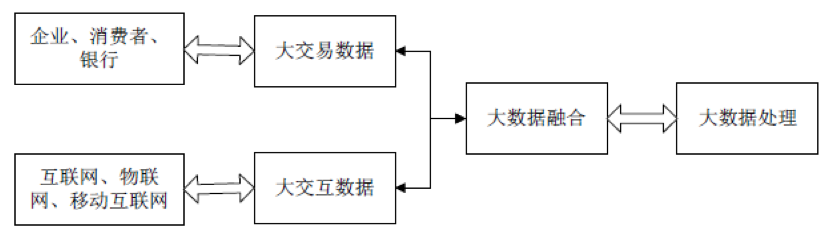
\includegraphics{images/example_figure2.png}
	\caption{XXXXXXXXXX}
\end{figure}

\clearpage
表示例
\begin{table}[!htb]
\centering
\caption{三种肌球蛋白/多糖混合凝胶的红外光谱数据}
\begin{tabular}{lcccc}
\hline
Treatment           & \multicolumn{4}{c}{FT-IR spectra numbers (cm$^{−1}$)} \\ \cline{2-5} 
                    & PK1        & PK2        & PK3        & PK4       \\ \hline
Myosin gel          & 3439       & —          & 1655       & 1106      \\
Myosin+ 1\% KCG gel & 3358       & 3006       & 1655       & 1131      \\
Myosin+ 1\% LBG gel & 3366       & 3006       & 1655       & 1106      \\
Myosin+ 1\% WSC gel & 3439       & —          & 1655       & 1106      \\ \hline
\end{tabular}
\end{table}

\begin{table}[!htb]
\centering
\caption{分栏表}
\begin{tabular}{ccccc}
\hline
年度                    & 产品  & 产量    & 销量    & 产值  \\ \hline
\multirow{2}{*}{2004} & 手机  & 11000 & 10000 & 500 \\
                      & 计算机 & 1100  & 1000  & 280 \\ \hline
\multirow{2}{*}{2005} & 手机  & 16000 & 13000 & 550 \\
                      & 计算机 & 2100  & 1500  & 320 \\ \hline
\end{tabular}
\end{table}





\begin{table}[!htb]
    \centering
    \caption{三种肌球蛋白/多糖混合凝胶的红外光谱数据}
    \begin{tabular}{lcccc}
        \hline
        Treatment           & \multicolumn{4}{c}{FT-IR spectra numbers (cm$^{−1}$)} \\ \cline{2-5} 
                            & PK1        & PK2        & PK3        & PK4       \\ \hline
        Myosin gel          & 3439       & —          & 1655       & 1106      \\
        Myosin+ 1\% KCG gel & 3358       & 3006       & 1655       & 1131      \\
        Myosin+ 1\% LBG gel & 3366       & 3006       & 1655       & 1106      \\
        Myosin+ 1\% WSC gel & 3439       & —          & 1655       & 1106      \\ \hline
    \end{tabular}
\end{table}
% 插入参考文献
% =============参考文献===========
{
\clearpage % 分页
\phantomsection % 使得hyperref目录能够跳转到正确的位置
\addcontentsline{toc}{section}{参考文献} % 添加到目录中
\nocite{*} % 添加所有文献
%\bibliographystyle{gbt7714-2005} % 样式
\wuhao							%设置字号
\songti							%设置字体
\setlength{\baselineskip}{20pt} %20磅行距
\bibliographystyle{bib/gbt7714-2005} % 样式
\bibliography{bib/ref.bib}    % 文献数据库
}

% 插入致谢
% ============致谢=============
\begin{acknowledge}
    本论文是在指导老师XXXXXXXXXXXXXXXXXXXXXXXXXXXXXXXXXXXXXXXXXXXXXXXXXXXXXXXXXXXXXXXXXXXXXXXXXXXXXXXXXXXXXXXXXXX。
    
    XXXXXXXXXXXXXXXXXXXXXXXXXXXXXXXXXXXXXXXXXXXXXXXXXXXXXXXXXXXXXXXXXXXXXX。
\end{acknowledge}
% 插入附录
% ============附录,必要时=======
\begin{appendix}
    【说明:以下内容可放在附录之内:(1) 正文内过于冗长的公式推导;(2) 方便他人阅读所需的辅助性数学工具或表格;(3) 重复性数据和图表;(4) 论文使用的主要符号的意义和单位;(5) 程序说明和程序全文。可按"附录1  XXX"、"附录2  XXX"、……,分章书写。如无需附录,请删除此页。】
\end{appendix}

\end{document}
